%\PassOptionsToPackage{landscape}{geometry}
\documentclass[aspectratio=169]{beamer}

\usepackage{bm}

%\usepackage{graphics}
\usepackage{graphicx}
\usepackage{amsmath,amssymb,amsthm}
\usepackage{bm}
%\usepackage{subfigure}

\usepackage{xcolor}
\usepackage{colortbl}

\def\boldred#1{\color{red}\textbf{#1}}

\def\IC{\mathbb{C}}
\def\IF{\mathbb{F}}
\def\II{\mathbb{I}}
\def\IM{\mathbb{M}}
\def\IN{\mathbb{N}}
\def\IP{\mathbb{P}}
\def\IR{\mathbb{R}}
\def\IZ{\mathbb{Z}}

\def\ba{\mathbf{a}}
\def\bb{\mathbf{b}}
\def\bc{\mathbf{c}}
\def\be{\mathbf{e}}
\def\bg{\mathbf{g}}
\def\bh{\mathbf{h}}
\def\bi{\mathbf{i}}
\def\bj{\mathbf{j}}
\def\bk{\mathbf{k}}
\def\bn{\mathbf{n}}
\def\bp{\mathbf{p}}
\def\br{\mathbf{r}}
\def\bs{\mathbf{s}}
\def\bu{\mathbf{u}}
\def\bv{\mathbf{v}}
\def\bw{\mathbf{w}}
\def\bx{\mathbf{x}}
\def\by{\mathbf{y}}
\def\bz{\mathbf{z}}

\def\bB{\mathbf{B}}
\def\bD{\mathbf{D}}
\def\bF{\mathbf{F}}
\def\bG{\mathbf{G}}
\def\bN{\mathbf{N}}
\def\bR{\mathbf{R}}
\def\bS{\mathbf{S}}
\def\bT{\mathbf{T}}
\def\b0{\mathbf{0}}

\bmdefine{\bmu}{\bm{\mu}}

\def\A{\mathcal{A}}
\def\B{\mathcal{B}}
\def\C{\mathcal{C}}
\def\D{\mathcal{D}}
\def\E{\mathcal{E}}
\def\F{\mathcal{F}}
\def\G{\mathcal{G}}
\def\I{\mathcal{I}}
\def\L{\mathcal{L}}
\def\M{\mathcal{M}}
\def\N{\mathcal{N}}
\def\P{\mathcal{P}}
\def\R{\mathcal{R}}
\def\S{\mathcal{S}}
\def\T{\mathcal{T}}
\def\U{\mathcal{U}}
\def\V{\mathcal{V}}

\def\nbOne{{\mathchoice {\rm 1\mskip-4mu l} {\rm 1\mskip-4mu l}
{\rm 1\mskip-4.5mu l} {\rm 1\mskip-5mu l}}}

\def\cov{\ensuremath{\mathsf{cov}}}
\def\Var{\ensuremath{\mathsf{Var}\ }}

\def\defword#1{\textbf{#1}\index{#1}}



%%%%%%%%%%%%%%%%%%%%%
%%%%%%%%%%%%%%%%%%%%%
%%
%%
%% NAVIGATION AND SECTIONING
%%
%%
%%%%%%%%%%%%%%%%%%%%%
%%%%%%%%%%%%%%%%%%%%%
\def\sgn{\ensuremath{\mathsf{sgn}}}

\newtheorem{proposition}[theorem]{Proposition}
\newtheorem{property}[theorem]{Property}
\newtheorem{importantproperty}[theorem]{Property}
\newtheorem{importanttheorem}[theorem]{Theorem}
%\newtheorem{lemma}[theorem]{Lemma}



\setbeamertemplate{navigation symbols}{}
\setbeamertemplate{footline}
{%
	\quad\insertsection\hfill p. \insertpagenumber\quad\mbox{}\vskip2pt
}
\usecolortheme{orchid}
\setbeamertemplate{theorems}[numbered]

\makeatletter
\newlength\beamerleftmargin
\setlength\beamerleftmargin{\Gm@lmargin}
\makeatother

%%%%%%%%%%%
% To have links to parts in the outline
\makeatletter
\AtBeginPart{%
	\addtocontents{toc}{\protect\beamer@partintoc{\the\c@part}{\beamer@partnameshort}{\the\c@page}}%
}
%% number, shortname, page.
\providecommand\beamer@partintoc[3]{%
	\ifnum\c@tocdepth=-1\relax
	% requesting onlyparts.
	\makebox[6em]{Chapter #1:} \textcolor{green!30!blue}{\hyperlink{#2}{#2}}
	\par
	\fi
}
\define@key{beamertoc}{onlyparts}[]{%
	\c@tocdepth=-1\relax
}
\makeatother%

\newcommand{\nameofthepart}{}
\newcommand{\nupart}[1]%
{   \part{#1}%
	\renewcommand{\nameofthepart}{#1}%
	{
		\setbeamercolor{background canvas}{bg=orange!50}
		\begin{frame}{#1}%\partpage 
			\hypertarget{\nameofthepart}{}\tableofcontents%
		\end{frame}
	}
}

% Beginning of a section
\AtBeginSection[]{
	{
		\setbeamercolor{background canvas}{bg=orange!10}
		\begin{frame}[noframenumbering,plain]
			\tableofcontents[currentsection,hideothersubsections]
		\end{frame}
		\addtocounter{page}{-1}
		%\addtocounter{framenumber}{-1} 
	}
}

% Beginning of a section
\AtBeginSubsection[]{
	{
		\setbeamercolor{background canvas}{bg=orange!10}
		\begin{frame}[noframenumbering,plain]
			\tableofcontents[sectionstyle=show/shaded,subsectionstyle=show/shaded/hide]
		\end{frame}
		\addtocounter{page}{-1}
		%\addtocounter{framenumber}{-1} 
	}
}




%%%%%%%%%%%%%%%%%%%%%
%%%%%%%%%%%%%%%%%%%%%
%%
%%
%% COLOURED ENVIRONMENTS
%%
%%
%%%%%%%%%%%%%%%%%%%%%
%%%%%%%%%%%%%%%%%%%%%
\newtheorem{proposition}[theorem]{Proposition}
\newtheorem{property}[theorem]{Property}
\newtheorem{importantproperty}[theorem]{Property}
\newtheorem{importanttheorem}[theorem]{Theorem}
%\newtheorem{lemma}[theorem]{Lemma}
%%%%%%% 
%% Definitions in yellow boxes
\usepackage{etoolbox}
\setbeamercolor{block title}{use=structure,fg=structure.fg,bg=structure.fg!05!bg}
\setbeamercolor{block body}{parent=normal text,use=block title,bg=block title.bg!20!bg}

\BeforeBeginEnvironment{definition}{%
	\setbeamercolor{block title}{fg=black,bg=yellow!20!white}
	\setbeamercolor{block body}{fg=black, bg=yellow!05!white}
}
\AfterEndEnvironment{definition}{
	\setbeamercolor{block title}{use=structure,fg=structure.fg,bg=structure.fg!20!bg}
	\setbeamercolor{block body}{parent=normal text,use=block title,bg=block title.bg!50!bg, fg=black}
}
\BeforeBeginEnvironment{importanttheorem}{%
	\setbeamercolor{block title}{fg=black,bg=red!20!white}
	\setbeamercolor{block body}{fg=black, bg=red!05!white}
}
\AfterEndEnvironment{importanttheorem}{
	\setbeamercolor{block title}{use=structure,fg=structure.fg,bg=structure.fg!20!bg}
	\setbeamercolor{block body}{parent=normal text,use=block title,bg=block title.bg!50!bg, fg=black}
}
\BeforeBeginEnvironment{importantproperty}{%
	\setbeamercolor{block title}{fg=black,bg=red!50!white}
	\setbeamercolor{block body}{fg=black, bg=red!30!white}
}
\AfterEndEnvironment{importantproperty}{
	\setbeamercolor{block title}{use=structure,fg=structure.fg,bg=structure.fg!20!bg}
	\setbeamercolor{block body}{parent=normal text,use=block title,bg=block title.bg!50!bg, fg=black}
}


% Colours for special pages
\def\extraContent{yellow!20}

% Allow to change slide colour
% From: https://tex.stackexchange.com/questions/8043/change-the-background-color-of-a-frame-in-beamer
\defbeamertemplate*{background canvas}{mydefault}{%
	\ifbeamercolorempty[bg]{background canvas}{}{\color{bg}\vrule width\paperwidth height\paperheight}% copied beamer default here
}
\defbeamertemplate*{background canvas}{bg}{%
	\color{lightgray!20}\vrule width\paperwidth height\paperheight% added bg color
}
\BeforeBeginEnvironment{frame}{%
	\setbeamertemplate{background canvas}[mydefault]%
}
\makeatletter
\define@key{beamerframe}{bg}[true]{%
	\setbeamertemplate{background canvas}[bg]%
}
\makeatother
% Use with
%\begin{frame}
% \frametitle{Normal}
%\end{frame} 
%\begin{frame}[bg]
% \frametitle{With bg}
%\end{frame}


% Vertical alignment on pages
% From: https://tex.stackexchange.com/questions/148365/how-do-i-ask-beamer-to-exactly-fill-up-a-slide
% Turn on with
% \stretchon
% (outside slide), and off with
% \stretchoff
\def\itemsymbol{$\blacktriangleright$}
%\def\itemsymbol{}
\let\svpar\par
\let\svitemize\itemize
\let\svenditemize\enditemize
\let\svitem\item
\let\svcenter\center
\let\svendcenter\endcenter
\let\svcolumn\column
\let\svendcolumn\endcolumn
\def\newitem{\renewcommand\item[1][\itemsymbol]{\vfill\svitem[##1]}}%
\def\newpar{\def\par{\svpar\vfill}}%
\newcommand\stretchon{%
	\newpar%
	\renewcommand\item[1][\itemsymbol]{\svitem[##1]\newitem}%
	\renewenvironment{itemize}%
	{\svitemize}{\svenditemize\newpar\par}%
	\renewenvironment{center}%
	{\svcenter\newpar}{\svendcenter\newpar}%
	\renewenvironment{column}[2]%
	{\svcolumn{##1}\setlength{\parskip}{\columnskip}##2}%
	{\svendcolumn\vspace{\columnskip}}%
}
\newcommand\stretchoff{%
	\let\par\svpar%
	\let\item\svitem%
	\let\itemize\svitemize%
	\let\enditemize\svenditemize%
	\let\center\svcenter%
	\let\endcenter\svendcenter%
	\let\column\svcolumn%
	\let\endcolumn\svendcolumn%
}
\newlength\columnskip
\columnskip 0pt

%%%%%%%%%%%%%%%%%
\usepackage{tikz}
\usetikzlibrary{shapes,arrows}
\usetikzlibrary{positioning}
\tikzstyle{cloud} = [draw, ellipse,fill=red!20, node distance=0.87cm,
minimum height=2em]
\tikzstyle{line} = [draw, -latex']
\usetikzlibrary{shapes.symbols,shapes.callouts,patterns}
\usetikzlibrary{calc,fit}
\usetikzlibrary{backgrounds}

\usetikzlibrary{decorations.pathmorphing,backgrounds,positioning,fit,petri}
\usetikzlibrary{automata}

% Index in the slides as well
\usepackage{makeidx}
\makeindex
\newenvironment{theindex}
 {\let\item\par
  %definitions for subitem etc
  }{}
\newcommand\indexspace{}

% Beginning of a section
\AtBeginSection[]{
	{
		\setbeamercolor{background canvas}{bg=orange!10}
		\begin{frame}[noframenumbering,plain]
			\framesubtitle{\nameofthepart Chapter \insertromanpartnumber \ -- \iteminsert{\insertpart}}
			\tableofcontents[currentsection,currentsubsection]
		\end{frame}
	\addtocounter{page}{-1}
	%\addtocounter{framenumber}{-1} 
	}
}


\title{Characteristing graphs}
\date{}

\begin{document}
\DeclareFontShape{OT1}{cmss}{b}{n}{<->ssub * cmss/bx/n}{} 
\begin{frame}
	\titlepage
\end{frame}

\stretchon

%%%%%%%%%%%%%%%%%%%%%
%%%%%%%%%%%%%%%%%%%%%
%%%%%%%%%%%%%%%%%%%%%
%%%%%%%%%%%%%%%%%%%%%
\begin{frame}{Why and how to characterise a graph}
Graphs are everywhere!

To compare graphs, understand their properties, we need ways to describe their shape and characteristics
\end{frame}


\begin{frame}{The global air transportation network}
	\bigskip
	{\centering
		\hspace*{-\beamerleftmargin}
		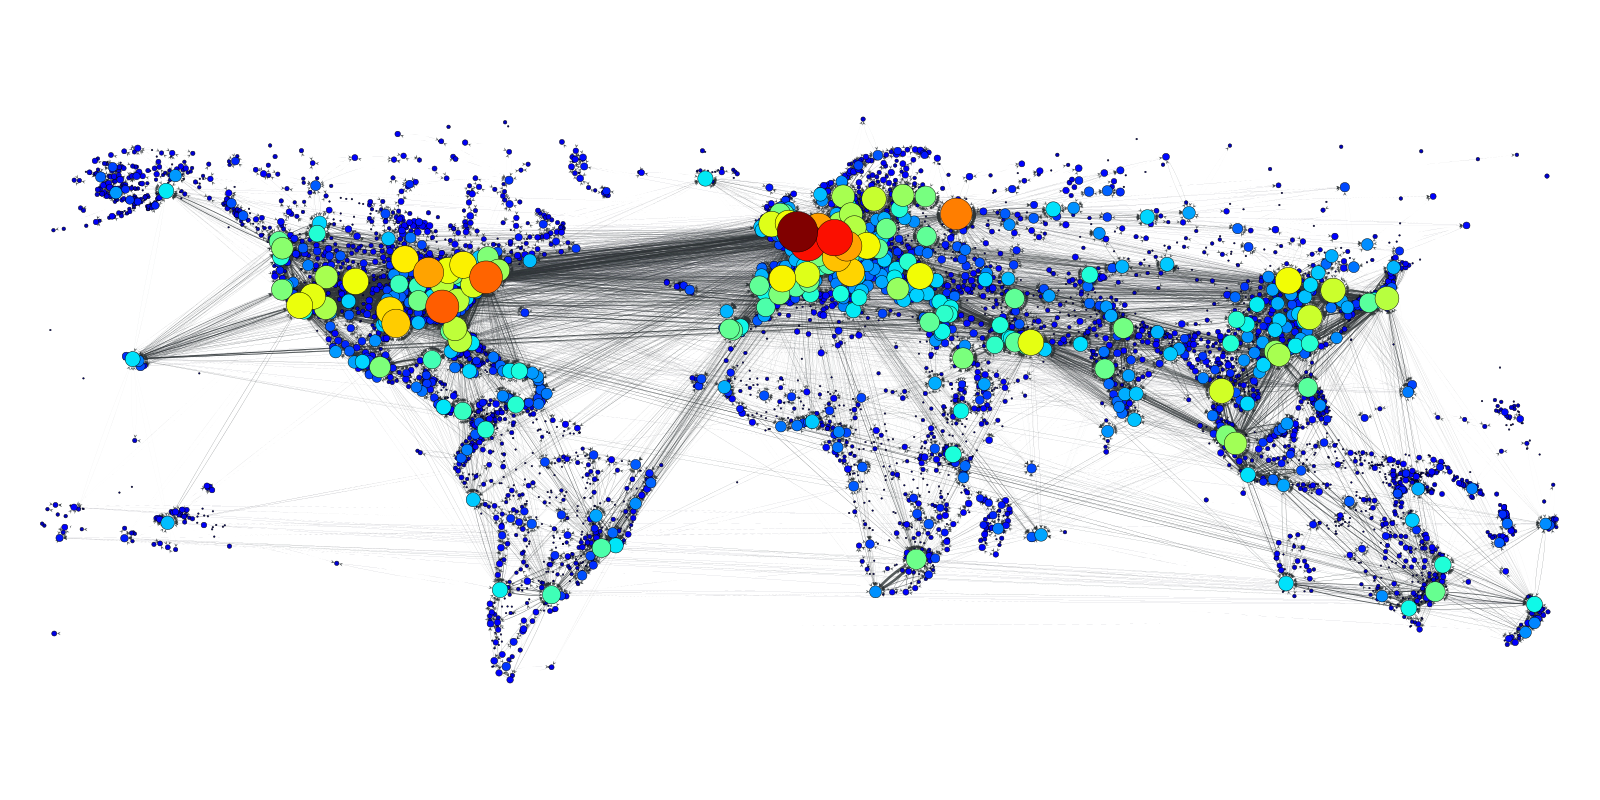
\includegraphics[width=\paperwidth]{FIGS_slides/world_graph-degree}
	}
\end{frame}

\begin{frame}{Example of spread of p-H1N1}
	\bigskip
	{\centering
		\hspace*{-\beamerleftmargin}
		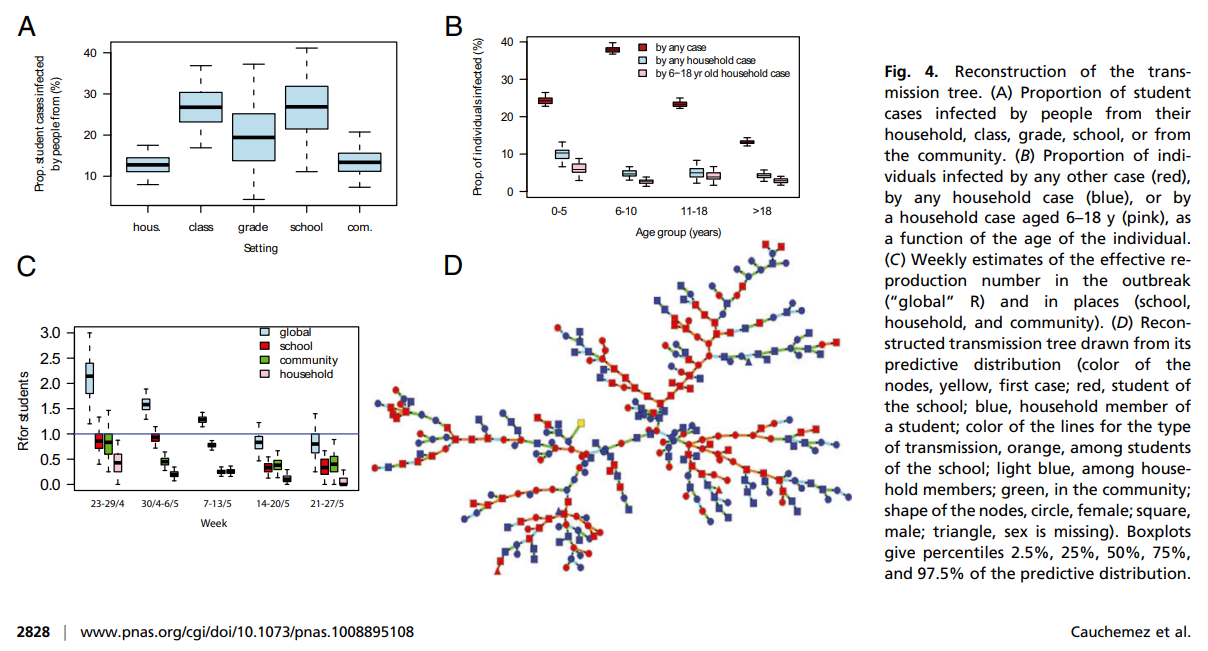
\includegraphics[width=\paperwidth]{FIGS_slides/Cauchemez_etal_H1N1}
	}
	\vskip0pt plus 1filll
	\tiny
	Role of social networks in shaping disease transmission during a community outbreak of 2009 H1N1 pandemic influenza, Cauchemez \emph{et al}, PNAS \textbf{108}(7):2825-2830 (2011)
\end{frame}

\begin{frame}{Example of spread of MERS}
	\begin{minipage}{0.8\textwidth}
		\hspace*{-\beamerleftmargin}
		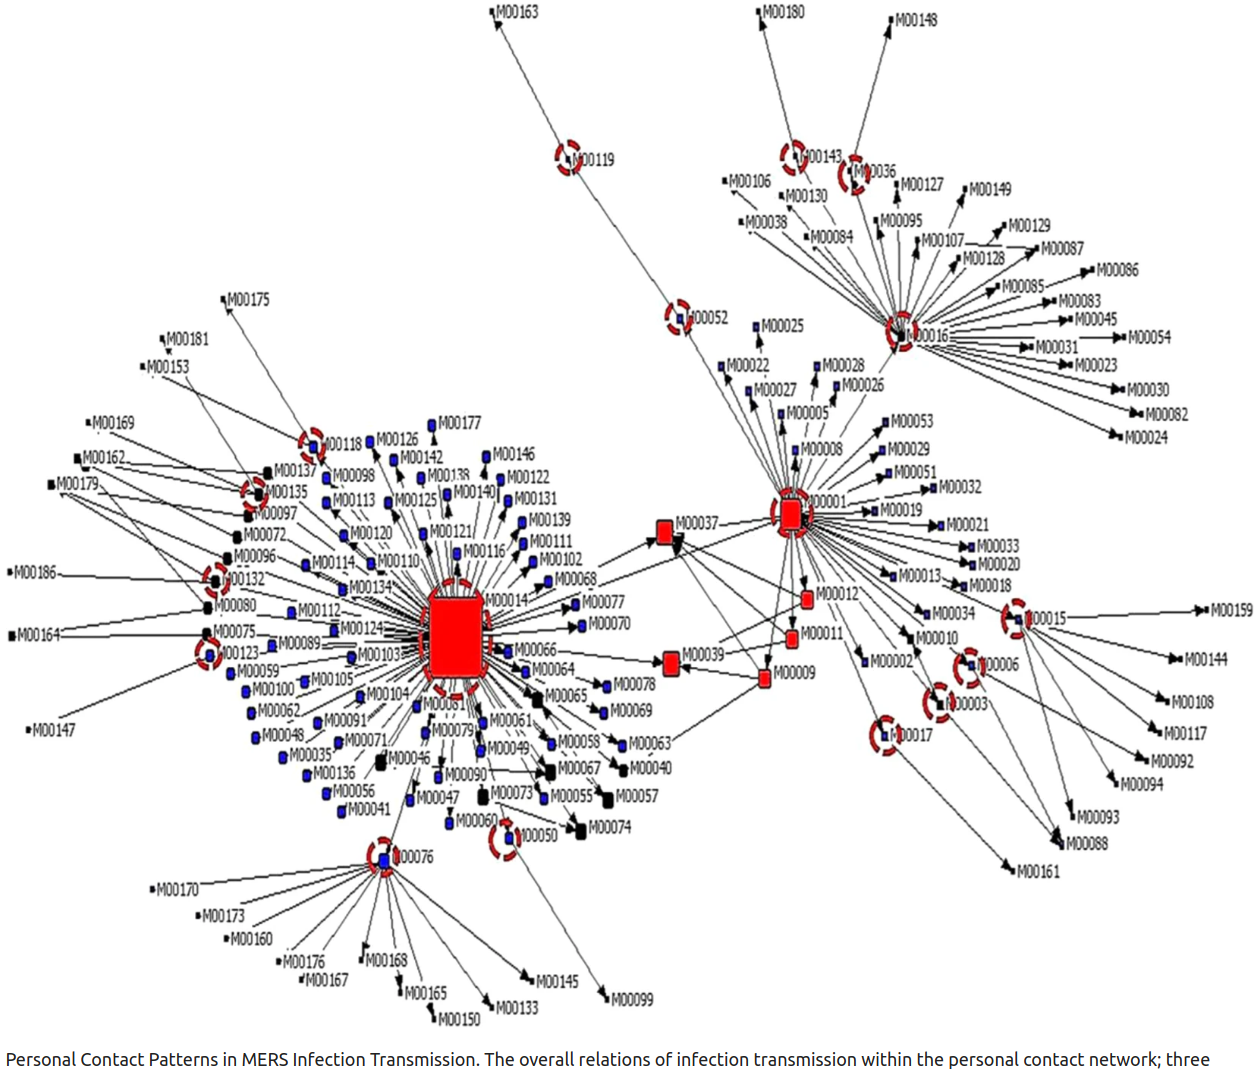
\includegraphics[height=\paperheight]{FIGS_slides/YangJung2015SouthKoreaMERS}
	\end{minipage}
	\begin{minipage}{0.18\textwidth}
	\tiny
	Topological dynamics of the 2015 South Korea MERS-CoV spread-on-contact networks, Yang \& Jung, Scientific Reports \textbf{10}:4327 (2020)
	\end{minipage}
\end{frame}


\begin{frame}
	Some ``measures'' concern the vertices, others the graph as a whole
	
	In all that follows, unless otherwise indicated, $G=(X,A)$ is a digraph. If undirected, we write $G=(X,E)$.
\end{frame}

%%%%%%%%%%%%%%%%%%%%%
%%%%%%%%%%%%%%%%%%%%%
%%%%%%%%%%%%%%%%%%%%%
%%%%%%%%%%%%%%%%%%%%%
\section{Measures specific to vertices}


%%%%%%%%%%%%%%%%%%%%%
%%%%%%%%%%%%%%%%%%%%%
\subsection{Centre of a graph}

\begin{frame}{Geodesic distance}
\begin{definition}[Geodesic distance]
For $x,y\in X$, the \defword{geodesic distance} $d(x,y)$ is the length of the shortest path from $x$ to $y$, with $d(x,y)=\infty$ if no such path exists
\end{definition}
\end{frame}

\begin{frame}
	\begin{minipage}{0.5\textwidth}
	\begin{itemize}
	\item $d(x_1,x_2)=1$
	\item $d(x_1,x_3)=2$
	\item $\cdots$
	\end{itemize}
	\vfill
	\[
	\begin{pmatrix}
	0 & 1 & 2 & 2 & 4 & 3 \\
	1 & 0 & 1 & 1 & 3 & 2 \\
	3 & 4 & 0 & 5 & 2 & 1 \\
	4 & 5 & 1 & 0 & 3 & 2 \\
	1 & 2 & 3 & 3 & 0 & 4 \\
	2 & 3 & 4 & 4 & 1 & 0
	\end{pmatrix}		
	\]		
	\end{minipage}
	\begin{minipage}{0.49\textwidth}
		\def\skip{2.75cm}
		\begin{tikzpicture}[scale=0.75,auto,
			cloud/.style={minimum width={width("N-1")+2pt},
				draw, ellipse},
			connected/.style={dotted,-}]
			%% Vertices
			\node [cloud] at (0,0) (x1) {$x_1$};
			\node [cloud] at (1*\skip,1*\skip) (x2) {$x_2$};
			\node [cloud] at (2*\skip,1*\skip) (x3) {$x_3$};
			\node [cloud] at (1.5*\skip,0) (x4) {$x_4$};
			\node [cloud] at (3*\skip,0*\skip) (x5) {$x_5$};
			\node [cloud] at (3*\skip,1*\skip) (x6) {$x_6$};
			%% Arcs
			\path [line, thick,bend left] (x1) to (x2);
			\path [line, thick,bend left] (x2) to (x1);
			\path [line, thick, looseness=5] (x2) to (x2);
			\path [line, thick] (x2) to (x3);
			\path [line, thick] (x2) to (x4);
			\path [line, thick] (x4) to (x3);
			\path [line, thick, looseness=5, below] (x6) to (x6);
			\path [line, thick] (x6) to (x5);
			\path [line, thick] (x3) to (x6);
			\path [line, thick, bend left] (x5) to (x1);
			\end{tikzpicture}
\end{minipage}
\end{frame}

\begin{frame}
	\begin{minipage}{0.5\textwidth}
	\begin{itemize}
		\item $d(x_5,x_1)=\infty$
		\item $d(x_3,x_1)=\infty$
		\item $\cdots$
	\end{itemize}
	\vfill
	\[
	\begin{pmatrix}
		0 & 1 & 2 & 2 & 4 & 3 \\
		1 & 0 & 1 & 1 & 3 & 2 \\
		\infty & \infty & 0 & \infty & 2 & 1 \\
		\infty& \infty& 1 & 0 & 3 & 2 \\
		\infty& \infty & \infty & \infty & 0 & \infty \\
		\infty & \infty & \infty & \infty & 1 & 0
	\end{pmatrix}
	\]
	\end{minipage}
	\begin{minipage}{0.49\textwidth}
		\def\skip{2.75cm}
		\begin{tikzpicture}[scale=0.75,auto,
			cloud/.style={minimum width={width("N-1")+2pt},
				draw, ellipse},
			connected/.style={dotted,-}]
			%% Vertices
			\node [cloud] at (0,0) (x1) {$x_1$};
			\node [cloud] at (1*\skip,1*\skip) (x2) {$x_2$};
			\node [cloud] at (2*\skip,1*\skip) (x3) {$x_3$};
			\node [cloud] at (1.5*\skip,0) (x4) {$x_4$};
			\node [cloud] at (3*\skip,0*\skip) (x5) {$x_5$};
			\node [cloud] at (3*\skip,1*\skip) (x6) {$x_6$};
			%% Arcs
			\path [line, thick,bend left] (x1) to (x2);
			\path [line, thick,bend left] (x2) to (x1);
			\path [line, thick, looseness=5] (x2) to (x2);
			\path [line, thick] (x2) to (x3);
			\path [line, thick] (x2) to (x4);
			\path [line, thick] (x4) to (x3);
			\path [line, thick, looseness=5, below] (x6) to (x6);
			\path [line, thick] (x6) to (x5);
			\path [line, thick] (x3) to (x6);
			\end{tikzpicture}
	\end{minipage}
\end{frame}

\begin{frame}{Eccentricity}
\begin{definition}[Vertex eccentricity]
	The \textbf{eccentricity} $e(x)$ of vertex $x\in X$ is 
	\[
		e(x)=\max_{\stackrel{y\in X}{y\neq x}}d(x,y)
	\]
\end{definition}
\begin{minipage}{0.5\textwidth}
	\[
\begin{pmatrix}
	0 & 1 & 2 & 2 & \boldred{4} & 3 \\
	1 & 0 & 1 & 1 & \boldred{3} & 2 \\
	3 & 4 & 0 & \boldred{5} & 2 & 1 \\
	4 & \boldred{5} & 1 & 0 & 3 & 2 \\
	1 & 2 & 3 & 3 & 0 & \boldred{4} \\
	2 & 3 & \boldred{4} & \boldred{4} & 1 & 0
\end{pmatrix}		
\]
\end{minipage}
\begin{minipage}{0.49\textwidth}
	\def\skip{2.75cm}
	\begin{tikzpicture}[scale = 0.75,auto,
		cloud/.style={minimum width={width("N-1")+2pt},
			draw, ellipse},
		connected/.style={dotted,-}]
		%% Vertices
		\node [cloud] at (0,0) (x1) {$x_1$};
		\node [cloud] at (1*\skip,1*\skip) (x2) {$x_2$};
		\node [cloud] at (2*\skip,1*\skip) (x3) {$x_3$};
		\node [cloud] at (1.5*\skip,0) (x4) {$x_4$};
		\node [cloud] at (3*\skip,0*\skip) (x5) {$x_5$};
		\node [cloud] at (3*\skip,1*\skip) (x6) {$x_6$};
		%% Arcs
		\path [line, thick,bend left] (x1) to (x2);
		\path [line, thick,bend left] (x2) to (x1);
		\path [line, thick, looseness=5] (x2) to (x2);
		\path [line, thick] (x2) to (x3);
		\path [line, thick] (x2) to (x4);
		\path [line, thick] (x4) to (x3);
		\path [line, thick, looseness=5, below] (x6) to (x6);
		\path [line, thick] (x6) to (x5);
		\path [line, thick] (x3) to (x6);
		\path [line, thick, bend left] (x5) to (x1);
		\end{tikzpicture}
\end{minipage}
\end{frame}


\begin{frame}{Central points, radius and centre}
\begin{definition}[Central point]
	A \textbf{central point} of $G$ is a vertex $x_0$ with smallest eccentricity
\end{definition}
\vfill
\begin{definition}[Radius]
	The \textbf{radius} of $G$ is $\rho(G)=e(x_0)$, where $x_0$ is a centre of $G$
	In other words,
	\[
	\rho(G)=\min_{x\in X}e(x)
	\]
\end{definition}
\vfill
\begin{definition}[Centre]
The \textbf{centre} of $G$ is the set of vertices that are central points of $G$, i.e.,
\[
    \{x\in X: e(x)=\rho(G)\}
\]
\end{definition}
\end{frame}


\begin{frame}
	\begin{minipage}{0.5\textwidth}
	\[
\begin{pmatrix}
	0 & 1 & 2 & 2 & \boldred{4} & 3 \\
	\rowcolor{gray!95}
	1 & 0 & 1 & 1 & \boldred{3} & 2 \\
	3 & 4 & 0 & \boldred{5} & 2 & 1 \\
	4 & \boldred{5} & 1 & 0 & 3 & 2 \\
	1 & 2 & 3 & 3 & 0 & \boldred{4} \\
	2 & 3 & \boldred{4} & \boldred{4} & 1 & 0
\end{pmatrix}		
\]
%\vfill
Radius is 3, $x_2$ is a central point (the only one) and the centre is $\{x_2\}$
	\end{minipage}
	\begin{minipage}{0.49\textwidth}
		\def\skip{2.5cm}
		\begin{tikzpicture}[scale = 0.85,auto,
			cloud/.style={minimum width={width("N-1")+2pt},
				draw, ellipse},
			connected/.style={dotted,-}]
			%% Vertices
			\node [cloud] at (0,0) (x1) {$x_1$};
			\node [cloud, fill=gray!20] at (1*\skip,1*\skip) (x2) {$x_2$};
			\node [cloud] at (2*\skip,1*\skip) (x3) {$x_3$};
			\node [cloud] at (1.5*\skip,0) (x4) {$x_4$};
			\node [cloud] at (3*\skip,0*\skip) (x5) {$x_5$};
			\node [cloud] at (3*\skip,1*\skip) (x6) {$x_6$};
			%% Arcs
			\path [line, thick,bend left] (x1) to (x2);
			\path [line, thick,bend left] (x2) to (x1);
			\path [line, thick, looseness=5] (x2) to (x2);
			\path [line, thick] (x2) to (x3);
			\path [line, thick] (x2) to (x4);
			\path [line, thick] (x4) to (x3);
			\path [line, thick, looseness=5, below] (x6) to (x6);
			\path [line, thick] (x6) to (x5);
			\path [line, thick] (x3) to (x6);
			\path [line, thick, bend left] (x5) to (x1);
			\end{tikzpicture}
	\end{minipage}
\end{frame}


%%%%%%%%%%%%%%%%%%%%%%
%%%%%%%%%%%%%%%%%%%%%%
\subsection{Centrality -- Betweenness and closeness}
\begin{frame}{How \emph{central} is a vertex?}
	\emph{Centrality} tries to answer the question: what are the most influent vertices? 
	
	We have seen central vertices and vertices on the periphery, let us consider two other measures of centrality
	\begin{itemize}
			\item Betweenness centrality
			\item Closeness centrality
	\end{itemize}
	Many other forms (we will come back to this, e.g., degree centrality)
\end{frame}

\begin{frame}{Betweenness}
\begin{definition}[Betweenness]
	$G=(X,U)$ a graph, $x\in X$. The \textbf{betweenness} of $v$ is
	\[
	b_\D(v)= \sum_{s\neq t\neq v  \in X} \frac{\sigma_{st}(v)}{\sigma_{st}}
	\]
	where
	\begin{itemize}
	\item $\sigma_{st}$ number of shortest geodesic paths from $s$ to $t$
	\item $\sigma_{st}(v)$ number of shortest geodesic paths from $s$ to $t$ through $v$
	\end{itemize}		
\end{definition}
\vfill
In other words
\begin{itemize}
	\item For each pair of vertices $(s,t)$, compute the shortest paths between them
	\item For each pair of vertices $(s,t)$, determine the fraction of shortest paths that pass through vertex $v$
	\item Sum this fraction over all pairs of vertices $(s,t)$
\end{itemize}
\end{frame}

\begin{frame}{Normalising betweenness}
	Betweenness may be normalized by dividing through the number of pairs of vertices not including $v$:
	\begin{itemize}
		\item for directed graphs, $(n-1)(n-2)$
		\item for undirected graphs, $(n-1)(n-2)/2$
	\end{itemize}
\end{frame}


\begin{frame}{Example of betweenness}
	\begin{minipage}{0.39\textwidth}
		{\tt distances(G, mode="out")}
		\[
			\begin{pmatrix}
				0 & 1 & 2 & 2 & 4 & 3 \\
				1 & 0 & 1 & 1 & 3 & 2 \\
				3 & 4 & 0 & 5 & 2 & 1 \\
				4 & 5 & 1 & 0 & 3 & 2 \\
				1 & 2 & 3 & 3 & 0 & 4 \\
				2 & 3 & 4 & 4 & 1 & 0
			\end{pmatrix}
		\]
		\end{minipage}
	\begin{minipage}{0.6\textwidth}
		\def\skip{2.75cm}
		\begin{tikzpicture}[scale = 0.85,
			every node/.style={transform shape},
			auto,
			cloud/.style={minimum width={width("N-1")+2pt},
				draw, ellipse},
			connected/.style={dotted,-}]
			%% Vertices
			\node [cloud] at (0,0) (x1) {$x_1$};
			\node [cloud] at (1*\skip,1*\skip) (x2) {$x_2$};
			\node [cloud] at (2*\skip,1*\skip) (x3) {$x_3$};
			\node [cloud] at (1.5*\skip,0) (x4) {$x_4$};
			\node [cloud] at (3*\skip,0*\skip) (x5) {$x_5$};
			\node [cloud] at (3*\skip,1*\skip) (x6) {$x_6$};
			%% Arcs
			\path [line, thick,bend left] (x1) to (x2);
			\path [line, thick,bend left] (x2) to (x1);
			\path [line, thick] (x2) to (x3);
			\path [line, thick] (x2) to (x4);
			\path [line, thick] (x4) to (x3);
			\path [line, thick] (x6) to (x5);
			\path [line, thick] (x3) to (x6);
			\path [line, thick, bend left] (x5) to (x1);
			\path [line, thick, looseness=5] (x2) to (x2);
			\path [line, thick, looseness=5, below] (x6) to (x6);
		\end{tikzpicture}
	\end{minipage}
\end{frame}


\begin{frame}{Number of shortest paths}
	Recall we found 
	{\tt distances(G, mode="out")}
	\[
		\mathcal{D} =
		\begin{pmatrix}
			0 & 1 & 2 & 2 & 4 & 3 \\
			1 & 0 & 1 & 1 & 3 & 2 \\
			3 & 4 & 0 & 5 & 2 & 1 \\
			4 & 5 & 1 & 0 & 3 & 2 \\
			1 & 2 & 3 & 3 & 0 & 4 \\
			2 & 3 & 4 & 4 & 1 & 0
		\end{pmatrix}
	\]
	\vfill
	To find the number of shortest paths between pairs of vertices, we can use powers of the adjacency matrix
	\vfill
	Write $\mathcal{D}=[d_{ij}]$, for a given $(i,j)$ ($i\neq j$), if $d_{ij}=k$, then pick the $(i,j)$ in $A^k$
\end{frame}

\begin{frame}
	We find
	\[
		\begin{pmatrix}
			0 & 1 & 1 & 1 & 1 & 1 \\
			1 & 0 & 1 & 1 & 1 & 1 \\
			1 & 1 & 0 & 1 & 1 & 1 \\
			1 & 1 & 1 & 0 & 1 & 1 \\
			1 & 1 & 1 & 1 & 0 & 1 \\
			1 & 1 & 1 & 1 & 1 & 0
		\end{pmatrix}
	\]
	\vfill
	Recall that betweenness of $v$ is
	\[
		b_\D(v)= \sum_{s\neq t\neq v  \in X} \frac{\sigma_{st}(v)}{\sigma_{st}}
	\]
	\vfill
	$\sigma_{st}$ (\# shortest paths from $s$ to $t$) is found in the matrix above
	\vfill
	What about $\sigma_{st}(v)$, \# of those shortest paths that go through $v$?
	\vfill
	We can use {\tt all\_shortest\_paths(G, from = s, to = t, mode = "out")}
\end{frame}


\begin{frame}{Example of betweenness}
	\begin{minipage}{0.35\textwidth}
		{\tt betweenness(G, directed = FALSE, normalized = TRUE)}

		Values shown in the vertices.
	\end{minipage}
	\begin{minipage}{0.6\textwidth}
		\def\skip{2.75cm}
		\begin{tikzpicture}[scale = 0.85,
			every node/.style={transform shape},
			auto,
			cloud/.style={minimum width={width("N-1")+2pt},
				draw, ellipse},
			connected/.style={dotted,-}]
			%% Vertices
			\node [cloud] at (0,0) (x1) {$0.5$};
			\node [cloud] at (1*\skip,1*\skip) (x2) {$0.5$};
			\node [cloud] at (2*\skip,1*\skip) (x3) {$0.45$};
			\node [cloud] at (1.5*\skip,0) (x4) {$0$};
			\node [cloud] at (3*\skip,0*\skip) (x5) {$0.45$};
			\node [cloud] at (3*\skip,1*\skip) (x6) {$0.45$};
			%% Arcs
			\path [line, thick,bend left] (x1) to (x2);
			\path [line, thick,bend left] (x2) to (x1);
			\path [line, thick] (x2) to (x3);
			\path [line, thick] (x2) to (x4);
			\path [line, thick] (x4) to (x3);
			\path [line, thick] (x6) to (x5);
			\path [line, thick] (x3) to (x6);
			\path [line, thick, bend left] (x5) to (x1);
			\path [line, thick, looseness=5] (x2) to (x2);
			\path [line, thick, looseness=5, below] (x6) to (x6);
		\end{tikzpicture}
	\end{minipage}
\end{frame}


\begin{frame}{Closeness}
	\begin{definition}
		$G=(X,U)$, $v\in X$. The \textbf{closeness} of $v$ is
		\[
		c_\D(v)=\frac{1}{n-1}\displaystyle \sum_{t\in X\setminus\{v\}}d_\D(v,t)
		\]
		i.e., mean geodesic distance between a vertex $v$ and all other vertices it has access to
		\vskip1cm 
		Another definition is
		\[
		c_\D(v)=\frac{1}{\displaystyle\sum_{t \in X\setminus\{v\}}d_\D(v,t)}
		\]				
	\end{definition}
\end{frame}

\begin{frame}{Example of (out) closeness}
	\vfill
	{\tt closeness(G, normalized = TRUE, mode=``out'')}
	\vfill
	\begin{center}
		\def\skip{2.75cm}
		\begin{tikzpicture}[scale = 0.85,
			every node/.style={transform shape},
			auto,
			cloud/.style={minimum width={width("N-1")+2pt},
				draw, ellipse},
			connected/.style={dotted,-}]
			%% Vertices
			\node [cloud] at (0,0) (x1) {$0.417$};
			\node [cloud] at (1*\skip,1*\skip) (x2) {$0.625$};
			\node [cloud] at (2*\skip,1*\skip) (x3) {$0.333$};
			\node [cloud] at (1.5*\skip,0) (x4) {$0.333$};
			\node [cloud] at (3*\skip,0*\skip) (x5) {$0.385$};
			\node [cloud] at (3*\skip,1*\skip) (x6) {$0.357$};
			%% Arcs
			\path [line, thick,bend left] (x1) to (x2);
			\path [line, thick,bend left] (x2) to (x1);
			\path [line, thick] (x2) to (x3);
			\path [line, thick] (x2) to (x4);
			\path [line, thick] (x4) to (x3);
			\path [line, thick] (x6) to (x5);
			\path [line, thick] (x3) to (x6);
			\path [line, thick, bend left] (x5) to (x1);
			\path [line, thick, looseness=5] (x2) to (x2);
			\path [line, thick, looseness=5, below] (x6) to (x6);
		\end{tikzpicture}
	\end{center}
\end{frame}
%%%%%%%%%%%%%%%%%%%%%%
%%%%%%%%%%%%%%%%%%%%%%
\subsection{Periphery of a graph}
\begin{frame}{Diametre and periphery of a graph}
\begin{definition}[Diametre of a graph]
The \textbf{diametre} of $G$ is 
\[
	\delta(G) = \max_{\stackrel{x,y\in X}{x\neq y}}d(x,y)
\]
or, in other words,
\[
	\delta(G)= \max_{x\in X}e(x)
\]
\end{definition}
\vfill
$\delta(G)<\infty$ $\iff$ $G$ strongly connected
\vfill
\begin{definition}[Periphery]
    The \textbf{periphery} of a graph is the set of vertices whose eccentricity achieves the diametre, i.e.,
    \[
        \{x\in X:e(x)=\delta(G)\}
    \]
\end{definition}
\end{frame}


\begin{frame}
		\begin{minipage}{0.5\textwidth}
	\[
\begin{pmatrix}
	0 & 1 & 2 & 2 & \boldred{4} & 3 \\
	1 & 0 & 1 & 1 & \boldred{3} & 2 \\
	\rowcolor{gray!95}
	3 & 4 & 0 & \boldred{5} & 2 & 1 \\
	\rowcolor{gray!95}
	4 & \boldred{5} & 1 & 0 & 3 & 2 \\
	1 & 2 & 3 & 3 & 0 & \boldred{4} \\
	2 & 3 & \boldred{4} & \boldred{4} & 1 & 0
\end{pmatrix}		
\]
Diametre is 5 and the periphery is $\{x_3,x_4\}$
	\end{minipage}
	\begin{minipage}{0.49\textwidth}
		\def\skip{2.5cm}
		\begin{tikzpicture}[scale = 0.85,auto,
			cloud/.style={minimum width={width("N-1")+2pt},
				draw, ellipse},
			connected/.style={dotted,-}]
			%% Vertices
			\node [cloud] at (0,0) (x1) {$x_1$};
			\node [cloud] at (1*\skip,1*\skip) (x2) {$x_2$};
			\node [cloud, fill=gray!20] at (2*\skip,1*\skip) (x3) {$x_3$};
			\node [cloud, fill=gray!20] at (1.5*\skip,0) (x4) {$x_4$};
			\node [cloud] at (3*\skip,0*\skip) (x5) {$x_5$};
			\node [cloud] at (3*\skip,1*\skip) (x6) {$x_6$};
			%% Arcs
			\path [line, thick,bend left] (x1) to (x2);
			\path [line, thick,bend left] (x2) to (x1);
			\path [line, thick, looseness=5] (x2) to (x2);
			\path [line, thick] (x2) to (x3);
			\path [line, thick] (x2) to (x4);
			\path [line, thick] (x4) to (x3);
			\path [line, thick, looseness=5, below] (x6) to (x6);
			\path [line, thick] (x6) to (x5);
			\path [line, thick] (x3) to (x6);
			\path [line, thick, bend left] (x5) to (x1);
			\end{tikzpicture}
		\end{minipage}	
	\begin{definition}[{Antipodal vertices}]
			A pair of vertices $x$ and $y$ are \defword{antipodal} if they satisfy $d(x,y)=\delta(G)$.
	\end{definition}
\end{frame}


%%%%%%%%%%%%%%%%%%%%%%%%
%%%%%%%%%%%%%%%%%%%%%%%%
\subsection{Degree distribution}

\begin{frame}{Degree distribution}
	\begin{definition}[Arc incident to a vertex]
		If a vertex $x$ is the initial endpoint of an arc $u$, which is not a loop, the arc $u$ is \textbf{incident out of vertex} $x$ 
		\vskip0.2cm
		The number of arcs incident out of $x$ plus the number of loops attached to $x$ is denoted $d_G^+(x)$ and is the \textbf{outer demi-degree} of $x$
		\vskip0.2cm
		An arc \textbf{incident into vertex} $x$ and the \textbf{inner demi-degree} $d_G^-(x)$ are defined similarly
		\end{definition}
		\vfill
		\begin{definition}[Degree]
		The \textbf{degree} of vertex $x$ is the number of arcs with $x$ as an endpoint, each loop being counted twice. The degree of $x$ is denoted $d_G(x)=d_G^+(x)+d_G^-(x)$
		\vskip0.2cm
		If each vertex has the same degree, the graph is \textbf{regular}
	\end{definition}
\end{frame}

\begin{frame}
	\begin{definition}[{Isolated vertex}]
	A vertex of degree $0$ is \textbf{isolated}.
	\end{definition}
	\begin{definition}[{Average degree of $G$}]
	$d(G)=\frac{1}{|V|}\sum_{v\in V}deg_G(v)$.
	\end{definition}
	\begin{definition}[{Minimum degree of $G$}]
	$\delta(G)=\min \{deg_G(v)|v\in V\}$.
	\end{definition}
	\begin{definition}[{Maximum degree of $G$}]
	$\Delta(G)=\max \{deg_G(v)|v\in V\}$.
	\end{definition}
\end{frame}


\begin{frame}{Degrees in an undirected graph}
	\begin{minipage}{0.65\textwidth}
		\def\skip{2.75cm}
		\begin{tikzpicture}[scale=0.75,auto,
			cloud/.style={minimum width={width("N-1")+2pt},
				draw, ellipse},
			connected/.style={dotted,-}]
			%% Vertices
			\node [cloud] at (0,0) (x1) {$2$};
			\node [cloud] at (1*\skip,1*\skip) (x2) {$3$};
			\node [cloud] at (2*\skip,1*\skip) (x3) {$3$};
			\node [cloud] at (1.5*\skip,0) (x4) {$2$};
			\node [cloud] at (3*\skip,0*\skip) (x5) {$2$};
			\node [cloud] at (3*\skip,1*\skip) (x6) {$2$};
			%% Arcs
			\draw [thick] (x1) --  (x2);
			\draw [thick] (x2) --  (x3);
			\draw [thick] (x2) --  (x4);
			\draw [thick] (x3) --  (x6);
			\draw [thick] (x4) --  (x3);
			\draw [thick] (x6) --  (x5);
			\draw (x5) to[thick, out=-150, in=-30] (x1);
			\end{tikzpicture}
	\end{minipage}
	\begin{minipage}{0.3\textwidth}
		Here, vertices are labelled using the degree
	\end{minipage}
\end{frame}


\begin{frame}{Degrees in a directed graph}
	\begin{minipage}{0.45\textwidth}
		\def\skip{2.75cm}
		\begin{tikzpicture}[scale = 0.65, 
			every node/.style={transform shape},
			auto,
			cloud/.style={minimum width={width("N-1")+2pt},
				draw, ellipse},
			connected/.style={dotted,-}]
			%% Vertices
			\node [cloud] at (0,0) (x1) {$\begin{matrix}d^+=1\\ d^-=2\end{matrix}$};
			\node [cloud] at (1*\skip,1*\skip) (x2) {$\begin{matrix}d^+=3\\ d^-=1\end{matrix}$};
			\node [cloud] at (2*\skip,1*\skip) (x3) {$\begin{matrix}d^+=1\\ d^-=2\end{matrix}$};
			\node [cloud] at (1.5*\skip,0) (x4) {$\begin{matrix}d^+=1\\ d^-=1\end{matrix}$};
			\node [cloud] at (3*\skip,0*\skip) (x5) {$\begin{matrix}d^+=1\\ d^-=1\end{matrix}$};
			\node [cloud] at (3*\skip,1*\skip) (x6) {$\begin{matrix}d^+=1\\ d^-=1\end{matrix}$};
			%% Arcs
			\path [line, thick,bend left] (x1) to (x2);
			\path [line, thick,bend left] (x2) to (x1);
			\path [line, thick] (x2) to (x3);
			\path [line, thick] (x2) to (x4);
			\path [line, thick] (x4) to (x3);
			\path [line, thick] (x6) to (x5);
			\path [line, thick] (x3) to (x6);
			\path [line, thick, bend left] (x5) to (x1);
			\end{tikzpicture}
	\end{minipage}
	\quad
	\begin{minipage}{0.45\textwidth}
		\def\skip{2.75cm}
		\begin{tikzpicture}[scale = 0.65, 
			every node/.style={transform shape},
			auto,
			cloud/.style={minimum width={width("N-1")+2pt},
				draw, ellipse},
			connected/.style={dotted,-}]
			%% Vertices
			\node [cloud] at (0,0) (x1) {$\begin{matrix}d^+=1\\ d^-=2\end{matrix}$};
			\node [cloud] at (1*\skip,1*\skip) (x2) {$\begin{matrix}d^+=4\\ d^-=2\end{matrix}$};
			\node [cloud] at (2*\skip,1*\skip) (x3) {$\begin{matrix}d^+=1\\ d^-=2\end{matrix}$};
			\node [cloud] at (1.5*\skip,0) (x4) {$\begin{matrix}d^+=1\\ d^-=1\end{matrix}$};
			\node [cloud] at (3*\skip,0*\skip) (x5) {$\begin{matrix}d^+=1\\ d^-=1\end{matrix}$};
			\node [cloud] at (3*\skip,1*\skip) (x6) {$\begin{matrix}d^+=2\\ d^-=2\end{matrix}$};
			%% Arcs
			\path [line, thick,bend left] (x1) to (x2);
			\path [line, thick,bend left] (x2) to (x1);
			\path [line, thick] (x2) to (x3);
			\path [line, thick] (x2) to (x4);
			\path [line, thick] (x4) to (x3);
			\path [line, thick] (x6) to (x5);
			\path [line, thick] (x3) to (x6);
			\path [line, thick, bend left] (x5) to (x1);
			\path [line, thick, looseness=5] (x2) to (x2);
			\path [line, thick, looseness=5] (x6) to (x6);
			\end{tikzpicture}
		\end{minipage}
\end{frame}


\begin{frame}{What to consider about degrees?}
	Degrees are often considered as a measure of popularity
	\vfill
	Often write $k(i)$ (or $k_i$) for ``degree of vertex $i$'', $k^-(i)$ and $k^+(i)$ for in- and out-degree
	\vfill
	\begin{itemize}
		\item Minimum and maximum degree
		\item Minimum and maximum in/out-degree. E.g., if you consider the global air transportation network and the in/out-degree of airports, in-degree is a measure of a location's ``popularity'' as a travel destination
		\item Range of degrees in a graph: are there large discrepancies in connectivity between vertices in the graph?
		\item Average degree (often denoted $\langle k\rangle$ because of physicists)
		\item Average in/out-degree
		\item Variance of the degrees or in/out-degrees
	\end{itemize}
\end{frame}



\begin{frame}
	\begin{itemize}
		\item Average (nearest) neighbour degree, to encode for \emph{preferential attachment} (one prefers to hang out with popular people)
		\[
			k_i^{nn} = \frac{1}{k(i)}\sum_{j\in\mathcal{N}(i)}k(j)
		\]
		or, in terms of the adjacency matrix $A=[a_{ij}]$,
		\[
			k_i^{nn} = \frac{1}{k(i)}\sum_{j}a_{ij}k(j)
		\]
		\item \emph{Excess degree}: take nearest neighbour degree but do not consider the edge/arc followed to get to the neighbour
		\item Degree, nearest neighbour and excess degree distributions
	\end{itemize}
\end{frame}


\begin{frame}{Degrees in {\tt igraph}}
	\begin{itemize}
		\item {\tt degree} gives the degrees of the vertices
		\item {\tt degree\_distribution} gives numeric vector of the same length as the maximum degree plus one. The first element is the relative frequency zero degree vertices, the second vertices with degree one, etc.
		\item {\tt knn} calculate the average nearest neighbor degree of the given vertices and the same quantity in the function of vertex degree
		\item {\tt strength} sums up the edge weights of the adjacent edges for each vertex
	\end{itemize}
\end{frame}

\begin{frame}{Degree from adjacency matrix}
	Suppose adjacency matrix take the form $A=[a_{ij}]$ with $a_{ij}=1$ if there is an arc from the vertex indexed $i$ to the vertex indexed $j$ and 0 otherwise. (Could be the other way round, using $A^T$, just make sure)
	\vfill
	Let $\be=(1,\ldots,1)^T$ be the vector of all ones 
	\vfill
	$A\be=(d_G^+(1),\ldots,d_G^+(1))^T$ (out-degree)
	\vfill
	$\be^TA=(d_G^-(1),\ldots,d_G^-(1))$ (in-degree)
\end{frame}


%%%%%%%%%%%%%%%%%%%%%%%%
%%%%%%%%%%%%%%%%%%%%%%%%
%%%%%%%%%%%%%%%%%%%%%%%%
%%%%%%%%%%%%%%%%%%%%%%%%
\section{Measures at the graph level}
%%%%%%%%%%%%%%%%%%%%%%%%
%%%%%%%%%%%%%%%%%%%%%%%%
\subsection{Circumference \& Girth}

\begin{frame}{Circumference}
\begin{definition}[Circumference]
    In an undirected (resp. directed) graph, the total number of edges (resp. arcs) in the longest cycle of graph $G$ is the \textbf{circumference} of $G$
\end{definition}
\begin{minipage}{0.5\textwidth}
	Circumference is 6.
\end{minipage}
\begin{minipage}{0.49\textwidth}
	\def\skip{2.5cm}
	\begin{tikzpicture}[scale = 0.85,auto,
		cloud/.style={minimum width={width("N-1")+2pt},
			draw, ellipse},
		connected/.style={dotted,-}]
		%% Vertices
		\node [cloud] at (0,0) (x1) {$x_1$};
		\node [cloud] at (1*\skip,1*\skip) (x2) {$x_2$};
		\node [cloud] at (2*\skip,1*\skip) (x3) {$x_3$};
		\node [cloud] at (1.5*\skip,0) (x4) {$x_4$};
		\node [cloud] at (3*\skip,0*\skip) (x5) {$x_5$};
		\node [cloud] at (3*\skip,1*\skip) (x6) {$x_6$};
		%% Arcs
		\path [line, thick,bend left, color=red] (x1) to (x2);
		\path [line, thick,bend left] (x2) to (x1);
		\path [line, thick] (x2) to (x3);
		\path [line, thick, color=red] (x2) to (x4);
		\path [line, thick, color=red] (x4) to (x3);
		\path [line, thick, color=red] (x6) to (x5);
		\path [line, thick, color=red] (x3) to (x6);
		\path [line, thick, bend left, color=red] (x5) to (x1);
		\end{tikzpicture}
\end{minipage}
\end{frame}


\begin{frame}{Girth}
\begin{definition}[Girth]
    The total number of edges in the shortest cycle of graph $G$ is the \textbf{girth} $g(G)$
\end{definition}
\begin{minipage}{0.3\textwidth}
	Girth is 2.
\end{minipage}
\begin{minipage}{0.69\textwidth}
	\def\skip{2.5cm}
	\begin{tikzpicture}[scale = 0.85,auto,
		cloud/.style={minimum width={width("N-1")+2pt},
			draw, ellipse},
		connected/.style={dotted,-}]
		%% Vertices
		\node [cloud] at (0,0) (x1) {$x_1$};
		\node [cloud] at (1*\skip,1*\skip) (x2) {$x_2$};
		\node [cloud] at (2*\skip,1*\skip) (x3) {$x_3$};
		\node [cloud] at (1.5*\skip,0) (x4) {$x_4$};
		\node [cloud] at (3*\skip,0*\skip) (x5) {$x_5$};
		\node [cloud] at (3*\skip,1*\skip) (x6) {$x_6$};
		%% Arcs
		\path [line, thick,bend left, color=red] (x1) to (x2);
		\path [line, thick,bend left, color=red] (x2) to (x1);
		\path [line, thick] (x2) to (x3);
		\path [line, thick] (x2) to (x4);
		\path [line, thick] (x4) to (x3);
		\path [line, thick] (x6) to (x5);
		\path [line, thick] (x3) to (x6);
		\path [line, thick, bend left] (x5) to (x1);
		\end{tikzpicture}
	\end{minipage}	
\end{frame}


%%%%%%%%%%%%%%%%%%%%%%%%
%%%%%%%%%%%%%%%%%%%%%%%%
\subsection{Graph density}

\begin{frame}{Completeness}
	\begin{definition}[{Complete undirected graph}]
		An undirected graph is complete if every two of its vertices are adjacent.
	\end{definition}
	\begin{definition}[{Complete digraph}]
		A digraph $D(V,A)$ is complete if $\forall u,v\in V$, $uv\in A$.
	\end{definition}
	\vfill
In case of simple graphs, completeness effectively means that ``information'' can be transmitted from every vertex to every other vertex quickly (1 step)
\vfill
It can be useful to know how far away we are from being complete
\end{frame}

\begin{frame}{Number of edges/arcs in a complete graph}
$G=(X,E)$ undirected and simple of order $n$ has at most
\[
	\frac {n(n-1)}{2}
\]
edges, while $G=(X,A)$ directed and simple of order $n$ has at most
\[
	n(n-1)
\]
arcs 
\end{frame}

\begin{frame}{Density of a graph}
	\begin{definition}[Density]
		The fraction of maximum number of edges or arcs present in the graph is the \textbf{density} of the graph.
	\end{definition}
If the graph has $p$ edges or arcs, then its density is, respectively,
\[
	\frac {2p}{n(n-1)}
\]
or 
\[
	\frac{p}{n(n-1)}
\]
\end{frame}

\begin{frame}{Example of density}
	\begin{minipage}{0.69\textwidth}
		\def\skip{2.75cm}
		\begin{tikzpicture}[scale = 0.85,auto,
			cloud/.style={minimum width={width("N-1")+2pt},
				draw, ellipse},
			connected/.style={dotted,-}]
			%% Vertices
			\node [cloud] at (0,0) (x1) {$x_1$};
			\node [cloud] at (1*\skip,1*\skip) (x2) {$x_2$};
			\node [cloud] at (2*\skip,1*\skip) (x3) {$x_3$};
			\node [cloud] at (1.5*\skip,0) (x4) {$x_4$};
			\node [cloud] at (3*\skip,0*\skip) (x5) {$x_5$};
			\node [cloud] at (3*\skip,1*\skip) (x6) {$x_6$};
			%% Arcs
			\path [line, thick,bend left] (x1) to (x2);
			\path [line, thick,bend left] (x2) to (x1);
			\path [line, thick] (x2) to (x3);
			\path [line, thick] (x2) to (x4);
			\path [line, thick] (x4) to (x3);
			\path [line, thick] (x6) to (x5);
			\path [line, thick] (x3) to (x6);
			\path [line, thick, bend left] (x5) to (x1);
			\end{tikzpicture}
		\end{minipage}
	\begin{minipage}{0.3\textwidth}
		Graph has order 6 and thus a max of 30 arcs. 
		Here, 8 arcs $\implies$ density 0.267
		\vfill 
		(26.7\% of arcs are present)	
	\end{minipage}
\end{frame}
	

%%%%%%%%%%%%%%%%%%%%%%%%
%%%%%%%%%%%%%%%%%%%%%%%%
\subsection{Graph connectivity}

\begin{frame}{Connectedness}
We have already seen connectedness (quasi- or strong in the oriented case)
\vfill
Connectedness is important in terms of characteristing graph properties, as it shows the capacity of the graph to convey information to all the members of the graph (the vertices)
\end{frame}


\begin{frame}
	\begin{definition}[Connected graph]
	A \textbf{connected graph} is a graph that contains a chain $\mu[x,y]$ for each pair $x,y$ of distinct vertices
	\end{definition}
	\vfill
	Denote $x\equiv y$ the relation  ``$x=y$, or $x\neq y$ and there exists a chain in $G$ connecting $x$ and $y$''. $\equiv$ is an equivalence relation since
	\begin{enumerate}
		\item $x\equiv y$ \hfill[reflexivity]
		\item $x\equiv y\implies y\equiv x$ \hfill[symmetry]
		\item $x\equiv y, y\equiv z\implies x\equiv z$ \hfill[transitivity]
	\end{enumerate}
	\begin{definition}[Connected component of a graph]
	The classes of the equivalence relation $\equiv$ partition $X$ into connected sub-graphs of $G$ called \textbf{connected components}
	\end{definition}
	\end{frame}
	
\begin{frame}{Articulation set} 
	\begin{definition}[Articulation set]
	For a connected graph, a set $A$ of vertices is called an \textbf{articulation set} (or a \textbf{cutset}) if the subgraph of $G$ generated by $X-A$ is not connected
	\end{definition}
	\vfill
	{\tt articulation\_points(G)} in {\tt igraph} (assumes the graph is undirected, makes it so if not)
\end{frame}

	
	\begin{frame}{Strongly connected graphs}
		$G=(X,U)$ connected. 
		A \textbf{path of length 0} is any sequence $\{x\}$ consisting of a single vertex $x\in X$
		\vfill
		For $x,y\in X$, let $x\equiv y$ be the relation ``there is a path $\mu_1[x,y]$ from $x$ to $y$ as well as a path $\mu_2[y,x]$ from $y$ to $x$''. This is an equivalence relation (it is reflexive, symmetric and transitive)
		\vfill
		\begin{definition}[Strong components]\label{def:strong_components}
		Sets of the form 
		\[
		A(x_0)=\{x:x\in X, x\equiv x_0\}	
		\]
		are equivalence classes; they partition $X$ and are the \textbf{strongly connected components} of $G$	
		\end{definition}
		\vfill
		\begin{definition}[Strongly connected graph]
		\label{def:strongly_connected_graph}
		$G$ \textbf{strongly connected} if it has a single strong component
		\end{definition}
\end{frame}
		

\begin{frame}
	\begin{definition}[Minimally connected graph]
	$G$ is \textbf{minimally connected} if it is strongly connected and removal of any arc destroys strong-connectedness
	\end{definition}
	\vfill
	\begin{definition}[Contraction]
	$G=(X,U)$. The \textbf{contraction} of the set $A\subset X$ of vertices consists in replacing $A$ by a single vertex $a$ and replacing each arc into (resp. out of) $A$ by an arc with same index into (resp. out of) $a$
	\end{definition}
\end{frame}
	
		
\begin{frame}{Quasi-strong connectedness}
	\begin{definition}[Quasi-strong connectedness]
	$G$ \textbf{quasi-strongly connected} if $\forall x,y\in X$, exists $z\in X$ (denoted $z(x,y)$ to emphasize dependence on $x,y$) from which there is a path to $x$ and a path to $y$
	\end{definition}
	\vfill
	Strongly connected $\implies$ quasi-strongly connected (take $z(x,y)=x$); converse not true
	\vfill
	Quasi-strongly connected $\implies$ connected
	\vfill
	\begin{lemma}
	$G=(X,U)$ has a root $\iff$ $G$ quasi-strongly connected
	\end{lemma}
\end{frame}

\begin{frame}{Weak-connectedness}
\begin{definition}[Weakly connected graph]
	$G=(X,U)$ \textbf{weakly connected} if $G=(X,E)$ connected, where $E$ is obtained from $U$ by ignoring the direction of arcs
\end{definition}
\vfill
	\begin{minipage}{0.4\textwidth}
		\def\skip{2.75cm}
		\begin{tikzpicture}[scale=0.5,auto,
			cloud/.style={minimum width={width("N-1")+2pt},
				draw, ellipse},
			connected/.style={dotted,-}]
			%% Vertices
			\node [cloud] at (0,0) (x1) {$x_1$};
			\node [cloud] at (1*\skip,1*\skip) (x2) {$x_2$};
			\node [cloud] at (2*\skip,1*\skip) (x3) {$x_3$};
			\node [cloud] at (1.5*\skip,0) (x4) {$x_4$};
			\node [cloud] at (3*\skip,0*\skip) (x5) {$x_5$};
			\node [cloud] at (3*\skip,1*\skip) (x6) {$x_6$};
			%% Arcs
			\path [line, thick,bend left] (x1) to (x2);
			\path [line, thick,bend left] (x2) to (x1);
			\path [line, thick] (x2) to (x3);
			\path [line, thick] (x2) to (x4);
			\path [line, thick] (x4) to (x3);
			\path [line, thick] (x6) to (x5);
			\path [line, thick] (x3) to (x6);
			\end{tikzpicture}
		\end{minipage}
		$\implies$
	\begin{minipage}{0.4\textwidth}
		\def\skip{2.75cm}
		\begin{tikzpicture}[scale=0.65,auto,
			cloud/.style={minimum width={width("N-1")+2pt},
				draw, ellipse},
			connected/.style={dotted,-}]
			%% Vertices
			\node [cloud] at (0,0) (x1) {$x_1$};
			\node [cloud] at (1*\skip,1*\skip) (x2) {$x_2$};
			\node [cloud] at (2*\skip,1*\skip) (x3) {$x_3$};
			\node [cloud] at (1.5*\skip,0) (x4) {$x_4$};
			\node [cloud] at (3*\skip,0*\skip) (x5) {$x_5$};
			\node [cloud] at (3*\skip,1*\skip) (x6) {$x_6$};
			%% Arcs
			\draw [thick] (x1) --  (x2);
			\draw [thick] (x2) --  (x3);
			\draw [thick] (x2) --  (x4);
			\draw [thick] (x3) --  (x6);
			\draw [thick] (x4) --  (x3);
			\draw [thick] (x6) --  (x5);
			\end{tikzpicture}
		\end{minipage}
\end{frame}


\begin{frame}{Weak components}
Define for $x,y\in X$ the relation $x\equiv y$ as ``$x=y$ or $x\neq y$ and there is a chain in $G$ connecting $x$ and $y$'' [like for components in an undirected graph, except the graph is directed here]
\vfill
This defines an equivalence relation
\begin{definition}[Weak components]
Sets of the form 
\[
	A(x_0)=\{x:x\in X, x\equiv x_0\}
\]
are equivalence classes partitioning $X$ into the \textbf{weakly connected components} of $G$
\end{definition}
\vfill
$G=(X,U)$ is weakly connected if there is a single weak component
\end{frame}


\begin{frame}{Components in {\tt igraph}}
\begin{itemize}
	\item {\tt is\_connected} decides whether the graph is weakly or strongly connected
	\item {\tt components} finds the maximal (weakly or strongly) connected components of a graph
	\item {\tt count\_components} does almost the same as components but returns only the number of clusters found instead of returning the actual clusters
	\item {\tt component\_distribution} creates a histogram for the maximal connected component sizes
	\item {\tt decompose} creates a separate graph for each component of a graph
	\item {\tt subcomponent} finds all vertices reachable from a given vertex, or the opposite: all vertices from which a given vertex is reachable via a directed path
\end{itemize}
\end{frame}
	
%%%%%%%%%%%%%%%%%%%%%%%%
%%%%%%%%%%%%%%%%%%%%%%%%
\subsection{Cliques}

\begin{frame}{Cliques}
	\begin{definition}[Clique in undirected graphs]
		$G=(X,E)$ a simple undirected graph. A \textbf{clique} is a subgraph $G'$ of $G$ such that all vertices in $G'$ are adjacent
	\end{definition}
	\begin{definition}[$n$-clique]
		A simple, complete graph on $n$ vertices is called an $n$-\textbf{clique} and is often denoted $K_n$
	\end{definition}
	\begin{definition}[Clique in directed graphs]
		$G=(X,U)$ a simple directed graph. A \textbf{clique} is a subgraph $G'$ of $G$ such that all vertices in $G'$ are mutually adjacent
	\end{definition}
	\begin{definition}[Maximal clique]
		A \textbf{maximal clique} is a clique that cannot be extended by adding another adjacent vertex
	\end{definition}
\end{frame}

\begin{frame}
	\begin{minipage}{0.45\textwidth}
		\def\skip{2.75cm}
		\begin{tikzpicture}[scale = 0.65,auto,
			cloud/.style={minimum width={width("N-1")+2pt},
				draw, ellipse},
			connected/.style={dotted,-}]
			%% Vertices
			\node [cloud, color=red] at (0,0) (x1) {$x_1$};
			\node [cloud, color=red] at (1*\skip,1*\skip) (x2) {$x_2$};
			\node [cloud] at (2*\skip,1*\skip) (x3) {$x_3$};
			\node [cloud] at (1.5*\skip,0) (x4) {$x_4$};
			\node [cloud] at (3*\skip,0*\skip) (x5) {$x_5$};
			\node [cloud] at (3*\skip,1*\skip) (x6) {$x_6$};
			%% Arcs
			\path [line, thick,bend left, color=red] (x1) to (x2);
			\path [line, thick,bend left, color=red] (x2) to (x1);
			\path [line, thick] (x2) to (x3);
			\path [line, thick] (x2) to (x4);
			\path [line, thick] (x4) to (x3);
			\path [line, thick] (x6) to (x5);
			\path [line, thick] (x3) to (x6);
			\path [line, thick, bend left] (x5) to (x1);
			\end{tikzpicture}
	\end{minipage}
	\quad
	\begin{minipage}{0.45\textwidth}
		\def\skip{2.75cm}
		\begin{tikzpicture}[scale=0.65,auto,
			cloud/.style={minimum width={width("N-1")+2pt},
				draw, ellipse},
			connected/.style={dotted,-}]
			%% Vertices
			\node [cloud] at (0,0) (x1) {$x_1$};
			\node [cloud, color=red] at (1*\skip,1*\skip) (x2) {$x_2$};
			\node [cloud, color=red] at (2*\skip,1*\skip) (x3) {$x_3$};
			\node [cloud, color=red] at (1.5*\skip,0) (x4) {$x_4$};
			\node [cloud] at (3*\skip,0*\skip) (x5) {$x_5$};
			\node [cloud] at (3*\skip,1*\skip) (x6) {$x_6$};
			%% Arcs
			\draw [thick] (x1) --  (x2);
			\draw [thick, color=red] (x2) --  (x3);
			\draw [thick, color=red] (x2) --  (x4);
			\draw [thick] (x3) --  (x6);
			\draw [thick, color=red] (x4) --  (x3);
			\draw [thick] (x6) --  (x5);
			\draw (x5) to[thick, out=-150, in=-30] (x1);
			\end{tikzpicture}
		\end{minipage}	
\end{frame}


\begin{frame}{Cliques in {\tt igraph}}
\begin{itemize}
	\item {\tt cliques} find all complete subgraphs in the input graph, obeying the size limitations given in the min and max arguments
	\item {\tt largest\_cliques} finds all largest cliques in the input graph
	\item {\tt max\_cliques} finds all maximal cliques in the input graph (The largest cliques are always maximal, but a maximal clique is not necessarily the largest)
	\item {\tt count\_max\_cliques} counts the maximal cliques
	\item {\tt clique\_num} calculates the size of the largest clique(s)
\end{itemize}
\end{frame}
	
	
%%%%%%%%%%%%%%%%%%
%%%%%%%%%%%%%%%%%%
\subsection{$k$-cores}

\begin{frame}{$k$-core}
	\begin{definition}[$k$-core of a graph]
		$G=(X,U)$ a graph. The $\mathbf{k}$-\textbf{core} of $G$ is a maximal subgraph in which each vertex has degree at least $k$
	\end{definition}
	\vfill
	\begin{definition}[Coreness of a vertex]
		$G=(X,U)$ a graph, $x\in X$. The \textbf{coreness} of $x$ is $k$ if $x$ belongs to the $k$-core of $G$ but not to the $k+1$ core of $G$
	\end{definition}
	\vfill
	For directed graphs, in-cores or out-cores depending on whether in-degree or out-degree is used
	\vfill
	In {\tt igraph}: {\tt coreness}
\end{frame}


\begin{frame}{Coreness in the directed case}
	\begin{center}
		\def\skip{2.75cm}
		\begin{tikzpicture}[scale = 0.85,auto,
			cloud/.style={minimum width={width("N-1")+2pt},
				draw, ellipse},
			connected/.style={dotted,-}]
			%% Vertices
			\node [cloud] at (0,0) (x1) {$x_1$};
			\node [cloud] at (1*\skip,1*\skip) (x2) {$x_2$};
			\node [cloud] at (2*\skip,1*\skip) (x3) {$x_3$};
			\node [cloud] at (1.5*\skip,0) (x4) {$x_4$};
			\node [cloud] at (3*\skip,0*\skip) (x5) {$x_5$};
			\node [cloud] at (3*\skip,1*\skip) (x6) {$x_6$};
			%% Arcs
			\path [line, thick,bend left] (x1) to (x2);
			\path [line, thick,bend left] (x2) to (x1);
			\path [line, thick] (x2) to (x3);
			\path [line, thick] (x2) to (x4);
			\path [line, thick] (x4) to (x3);
			\path [line, thick] (x6) to (x5);
			\path [line, thick] (x3) to (x6);
			\path [line, thick, bend left] (x5) to (x1);
			\path [line, thick, looseness=5] (x2) to (x2);
			\path [line, thick, looseness=5, below] (x6) to (x6);
		\end{tikzpicture}
	\end{center}
	\vfill
	$G$ has only a 1-in-core and 1-out-core: there is no (maximal) subgraph	in which the in- or out-degree is larger than 1
\end{frame}

\begin{frame}{In-coreness in the directed case}
	\begin{minipage}{0.45\textwidth}
		\def\skip{2.75cm}
		\begin{tikzpicture}[scale = 0.65,auto,
			cloud/.style={minimum width={width("N-1")+2pt},
				draw, ellipse},
			connected/.style={dotted,-}]
			%% Vertices
			\node [cloud] at (0,0) (x1) {$x_1$};
			\node [cloud] at (1*\skip,1*\skip) (x2) {$x_2$};
			\node [cloud] at (2*\skip,1*\skip) (x3) {$x_3$};
			\node [cloud] at (1.5*\skip,0) (x4) {$x_4$};
			\node [cloud] at (3*\skip,0*\skip) (x5) {$x_5$};
			\node [cloud] at (3*\skip,1*\skip) (x6) {$x_6$};
			%% Arcs
			\path [line, thick,bend left] (x1) to (x2);
			\path [line, thick,bend left] (x2) to (x1);
			\path [line, thick,bend left] (x2) to (x3);
			\path [line, thick,bend left] (x3) to (x2);
			\path [line, thick] (x2) to (x4);
			\path [line, thick] (x4) to (x3);
			\path [line, thick] (x6) to (x5);
			\path [line, thick,bend left] (x3) to (x6);
			\path [line, thick,bend left] (x6) to (x3);
			\path [line, thick, bend left] (x5) to (x1);
			\path [line, thick, looseness=5] (x2) to (x2);
			\path [line, thick, looseness=5, below] (x6) to (x6);
		\end{tikzpicture}
	\end{minipage}
	$\implies$
	\begin{minipage}{0.45\textwidth}
		\def\skip{2.75cm}
		\begin{tikzpicture}[scale = 0.65,auto,
			cloud/.style={minimum width={width("N-1")+2pt},
				draw, ellipse},
			connected/.style={dotted,-}]
			%% Vertices
			\node [cloud] at (0,0) (x1) {$1$};
			\node [cloud, red] at (1*\skip,1*\skip) (x2) {$2$};
			\node [cloud, red] at (2*\skip,1*\skip) (x3) {$2$};
			\node [cloud] at (1.5*\skip,0) (x4) {$1$};
			\node [cloud] at (3*\skip,0*\skip) (x5) {$1$};
			\node [cloud, red] at (3*\skip,1*\skip) (x6) {$2$};
			%% Arcs
			\path [line, thick,bend left] (x1) to (x2);
			\path [line, thick,bend left] (x2) to (x1);
			\path [line, thick,bend left,red] (x2) to (x3);
			\path [line, thick,bend left,red] (x3) to (x2);
			\path [line, thick] (x2) to (x4);
			\path [line, thick] (x4) to (x3);
			\path [line, thick] (x6) to (x5);
			\path [line, thick,bend left,red] (x3) to (x6);
			\path [line, thick,bend left,red] (x6) to (x3);
			\path [line, thick, bend left] (x5) to (x1);
			\path [line, thick, looseness=5,red] (x2) to (x2);
			\path [line, thick, looseness=5,red, below] (x6) to (x6);
		\end{tikzpicture}
	\end{minipage}
\end{frame}

\begin{frame}{Coreness in the undirected case}
	\begin{minipage}{0.45\textwidth}
		\def\skip{2.75cm}
		\begin{tikzpicture}[scale=0.65,
			every node/.style={transform shape},
			auto,
			cloud/.style={minimum width={width("N-1")+2pt},
				draw, ellipse},
			connected/.style={dotted,-}]
			%% Vertices
			\node [cloud] at (0,0) (x1) {$2$};
			\node [cloud] at (1*\skip,1*\skip) (x2) {$2$};
			\node [cloud] at (2*\skip,1*\skip) (x3) {$2$};
			\node [cloud] at (1.5*\skip,0) (x4) {$2$};
			\node [cloud] at (3*\skip,0*\skip) (x5) {$2$};
			\node [cloud] at (3*\skip,1*\skip) (x6) {$2$};
			%% Arcs
			\draw [thick] (x1) --  (x2);
			\draw [thick] (x2) --  (x3);
			\draw [thick] (x2) --  (x4);
			\draw [thick] (x3) --  (x6);
			\draw [thick] (x4) --  (x3);
			\draw [thick] (x6) --  (x5);
			\draw (x5) to[thick, out=-150, in=-30] (x1);
			\draw [thick,looseness=5] (x2) to (x2);
			\draw [thick,looseness=5] (x6) to (x6);
		\end{tikzpicture}
	\end{minipage}	
	$\implies$
	\begin{minipage}{0.45\textwidth}
		\def\skip{2.75cm}
		\begin{tikzpicture}[scale=0.65,
			every node/.style={transform shape},
			auto,
			cloud/.style={minimum width={width("N-1")+2pt},
				draw, ellipse},
			connected/.style={dotted,-}]
			%% Vertices
			\node [cloud] at (0,0) (x1) {$2$};
			\node [cloud,red] at (1*\skip,1*\skip) (x2) {$3$};
			\node [cloud,red] at (2*\skip,1*\skip) (x3) {$3$};
			\node [cloud] at (1.5*\skip,0) (x4) {$2$};
			\node [cloud] at (3*\skip,0*\skip) (x5) {$2$};
			\node [cloud,red] at (3*\skip,1*\skip) (x6) {$3$};
			%% Arcs
			\draw [thick] (x1) --  (x2);
			\draw [thick,red] (x2) --  (x3);
			\draw [thick] (x2) --  (x4);
			\draw [thick,red] (x3) --  (x6);
			\draw [thick] (x4) --  (x3);
			\draw [thick] (x6) --  (x5);
			\draw (x5) to[thick, out=-150, in=-30] (x1);
			\draw [thick,looseness=5,red] (x2) to (x2);
			\draw [thick,looseness=5,red] (x3) to (x3);
			\draw [thick,looseness=5,red] (x6) to (x6);
		\end{tikzpicture}
	\end{minipage}	
\end{frame}

%%%%%%%%%%%%%%%%%%
%%%%%%%%%%%%%%%%%%
%%%%%%%%%%%%%%%%%%
%%%%%%%%%%%%%%%%%%



\end{document}
